\chapter{Hauptteil}

\section{Design/Architektur}
Um eine Schnittstelle zwischen der Datenbankanwendung und dem Nutzer zu schaffen, existieren zwei verschiedene Anwendungen, welche über eine REST-API kommunizieren.

Im folgenden wird zu aller erst auf die Technologien der Datenbankanwendung eingegangen und danach auf die,des Clients. Auf die Funktion der Architektur wird im Abschnitt Implementierung weiter eingegangen. 

Beide Anwendungen bauen auf der Programmiersprache Java 8 auf.

\subsection{Technologie-Stack Datenbankanwendung}

Grundsätzlich besteht die Datenbankanwendung aus drei verschiedenen Technologie Layern, welche miteinander intern von unten nach oben und zurück kommunizieren und lässt sich somit einer Schichtenarchitektur zuordnen. 



\begin{figure}[h]
  \centering
  \begin{subfigure}[b]{1.0\textwidth}
    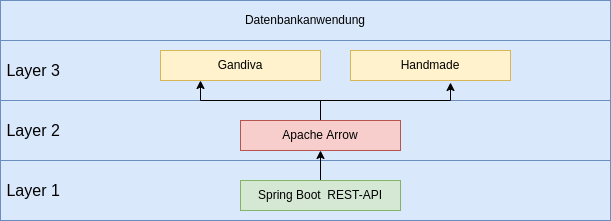
\includegraphics[width=1.0\linewidth]{img/layerarch}
  \end{subfigure}
  \caption{Technologie-Stack der DB-Anwendung}
  \label{graf_1}
\end{figure}

Im ersten Layer in \ref{graf_1} befindet sich das Spring-Boot Framework.
Dieses ist nötig um die Schnittstelle zwischen Client und Datenbankanwendung in Form einer Rest-Api sicher zu stellen. 
Über diese Rest-Api kann ein SQL-Dump mit verschiedensten Daten initialisiert werden, sowie Daten mithilfe von SQL-Queries abgefragt werden.

Die Anfragen werden dann mithilfe des Frameworks Arrow in Layer Zwei weiterverarbeitet. Dieser Layer Zwei kümmert sich um die Verwaltung der Daten im Speicher und ist das Herz der Datenbankanwendung. Über Arrow lassen sich die Daten in einem Spalten-Format im Hauptspeicher ablegen und aufrufen.

Im dritten Layer in \ref{graf_1} findet man das Framework Gandiva vor. 
Gandiva wird zum Filtern und zum Projizieren von den im Arrow-Format abgelegten Daten benutzt. Für den Fall das eine SQL-Query nicht mithilfe von Gandiva ausgewertet werden kann, kann hier eine Handmade-Implementierung genutzt werden.



\subsection{Technologie-Stack Clientanwendung}

Die Client-Anwendung basiert ebenfalls auf dem Spring-Boot Framework. Hier wird jedoch das Spring Shell Paket benutzt um eine interaktive Shell bereitstellen zu können.

Über die interaktive Shell kann eine Datenbank aus einem SQL-Dump initiliasiert werden oder einfache SQL-Queries versendet werden. Ebenfalls ist es möglich bestimmte Informationen über die Datenbank anzufragen.
Ziel der Datenbankanfragen ist es die nötigen Daten in einer Index-basierten Form zurückzuliefern, um später dann mithilfe von RDMA über die ebenfalls mitgelieferten Speicheradressen die Daten abfragen zu können.


\section{Implementierung}

Um die Implementierung möglichst Strukturiert zu beschreiben wird hier wieder die Datenbankanwendung und der Client getrennt betrachtet.
Im folgenden Teil wird auf die Umsetzung der Architektur/Designs eingegangen, sowie auf das Zusammenspiel der Komponenten,der Layer und Funktionen.
Da Gradle als build-Tool für die Anwendung benutzt wird lassen sich alle Technologien in der Anwendung im build.gradle File wieder finden. 


\section{Komponenten}

Für den Einstiegspunkt der Datenbankanwendung ist die Initialisierung einer Datenbank nötig. Bevor jedoch auf die verschiedenen Services der Anwendung eingegangen wird, müssen vorerst die einzelnen Datenmodelle beschrieben werden. 

\subsection{Modelle}
In der API/Datenbankanwendung existieren drei wichtige Modelle:

\begin{itemize}
 \item \textbf{Statement.java}: Dieses Modell wird als Datatransferobject behandelt. Statement enthält das SQL-Statement und wird mithilfe von Spring Boot aus dem jeweiligen Request des Clients ausgelesen und befüllt. Somit kommt über die Rest-API, die SQL-Query, in der Datenbankanwendung an und kann ausgewertet werden.
 \item \textbf{IndexResponse.java}: Wird von den verschiedenen Services, welche im folgenden Teil genauer beschrieben werden,befüllt. Das IndexResponse-Modell enthält die Speicheradressen im virtuellen Speicher und die verschiedenen Offset-Indices, falls ein Filter auf die Daten angewendet wurde. Ebenfalls enthält das Modell die verschiedenen Typen der Daten, um an die richtige Stelle im Speicher, mithilfe der Indices zu springen.
 \item \textbf{Table.java}: In diesem Modell liegen die Daten der Datenbank. Bei Initialisierung wird ein leeres VectorSchemaRoot-Objekt mithilfe eines Schemas angelegt. Dieses Objekt spiegelt das Grundgerüst der Datenbank wieder. Hier werden die Verschiedenen Spalten in Form von Vektoren gespeichert. Jeder Vektor ist einer Spalte aus dem SQL-Dump zuzuordnen.
\end{itemize}

\begin{figure}[h]
  \centering
  \begin{subfigure}[b]{1.0\textwidth}
    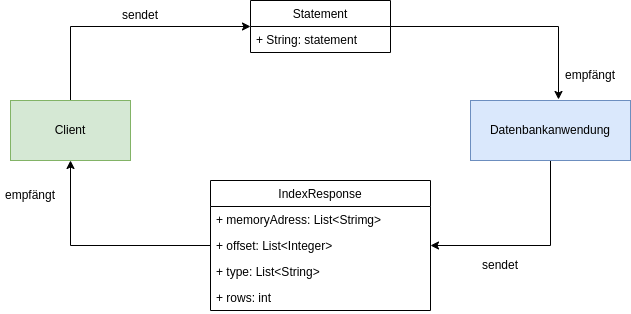
\includegraphics[width=1.0\linewidth]{img/sendrecieve}
  \end{subfigure}
  \caption{Modell-API-Kreislauf}
  \label{graf_2}
\end{figure}


In \ref{graf_2} ist das Zusammenspiel der Modelle dargestellt. Hier wird vom Client ein Statement gesendet und von der Datenbankanwendung mithilfe der Rest-API empfangen. Nach der Prozessierung des Statement erstellt die Datenbankanwendung eine IndexResponse und sendet diese dem Client zurück.





\subsection{Services}
Um eine Datenbank zu initialisieren oder ein SQL-Statement an diese schicken zu können, muss der Client, über eine Rest-API,das Backend anstoßen.
Da unter der reinen Datenbank eine Rest-API liegt, kann man über verschiedene Routen in dem \textbf{StatementController.java} diese ansteuern.


\subsubsection{StatementController}
Es existieren zwei wichtige Routen:

\begin{itemize}
 \item Get-Method: /initDatabase : Initialisierung eines SQL-Dumps,welcher in dem gleichen Ordner der Anwendung liegt
 \item Post-Method: /sendStatement: empfängt SQL-Statement vom Client aus und schickt eine IndexResponse zurück
\end{itemize}

Mithilfe dieser Routen kann über den StatementController in Form von einer Rest-Schnittstelle kommuniziert werden.
Wenn ein SQL-Dump über die Route initialisiert wird, erstellt der DumpReader-Service einen Table. (\ref{graf_3}). 


\subsubsection{DumpReader-Service}
Der DumpReader-Service ist für das lesen des SQL-Dumps zuständig. Er iteriert über jedes Statement in der Dump Datei,überprüft dieses und reagiert je noch Typ des Statements anders.
Findet man beispielsweise folgendes Statement im Kopf des SQL-Dumps,
\\

\begin{terminalblock}
  \begin{textcode}
CREATE TABLE `myTable` (
  `id` mediumint(8) unsigned NOT NULL auto_increment,
  `name` varchar(255) default NULL,
  `numberrange` mediumint default NULL,
  PRIMARY KEY (`id`)
) AUTO_INCREMENT=1;
  \end{textcode}
\end{terminalblock}\\
dann erkennt der DumpReader-Service das Create-Statement und legt ein neues Table-Objekt. Dieses muss jedoch ein spezifisches Schema erhalten,sowie die verschiedenen Spaltenfelder und deren Typ.
Diese Information erhält der Service aus dem SQL-Dump.
Das Statement wird mithilfe von JSQL geparsed.
Zu diesem Zeitpunkt unterstützt der DumpReader-Service nur die Typen:

\begin{itemize}
 \item Char
 \item VarChar
 \item mediumint
\end{itemize}

Da Apache Arrow seine eigenen Datentypen besitzt muss von den SQL-Datentypen,die in dem SQL-Dump vorhanden sind, zu den jeweiligen Apache Arrow Datentypen gemapped werden. 
Dieses Mapping wird durch die Methode \textbf{prepareField(String colName, String colDataType)} erreicht.
Diese Methode kann beliebig erweitert werden um weitere Datentypen zu unterstützen.\\
Nachdem das Tableobjekt erstellt wurde, iteriert der DumpReader-Service weiter über die Statements bis er ein Insert-Statement findet. Dieses Insert-Statement ist wichtig um den Table mit Daten zu füllen.
Ein Insert-Statement könnte beispielsweise so aussehen:\\

\begin{terminalblock}
  \begin{textcode}
INSERT INTO `myTable` (`name`,`numberrange`)
VALUES
  ("Oleg Estrada",4),
  ("Bevis Davenport",0),
  ("Ronan Tucker",9);
  \end{textcode}
\end{terminalblock}\\

Der DumpReader-Service erkennt nun das Insert-Statement und springt in die \textbf{prepareDataForMemory(String stmt,Table table)} Methode. Hier wird wieder mithilfe von JSQL das INSERT-Statement geparsed und in Datenstücke aufgespalten.
Da bei der Initialisierung der Datenbank ein Table-Objekt mit einem VectorSchemaRoot-Objekt und einem Schema erstellt wird,können hier die Daten aus dem Insert-Statement in die dazugehörigen Vektoren geschrieben werden.
Zusätzlich wird ein Indexvektor hochgezählt,welcher den Index des Eintrags abbildet.


\begin{figure}[h]
  \centering
  \begin{subfigure}[b]{1.0\textwidth}
    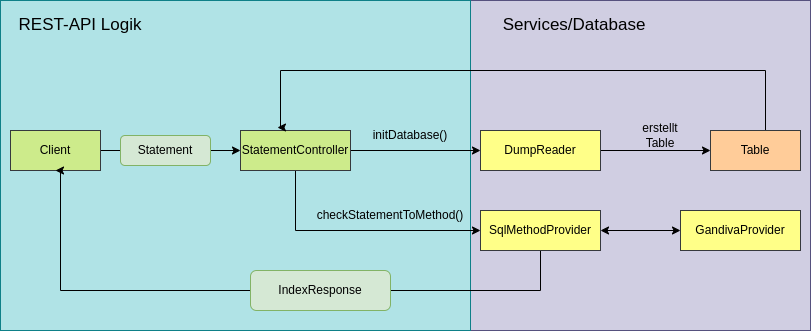
\includegraphics[width=1.0\linewidth]{img/logic}
  \end{subfigure}
  \caption{Überblick Rest-API/Services}
  \label{graf_3}
\end{figure}






